\documentclass[11pt, oneside]{article}   	% use "amsart" instead of "article" for AMSLaTeX format
\usepackage{geometry}                		% See geometry.pdf to learn the layout options. There are lots.
\geometry{letterpaper}                   		% ... or a4paper or a5paper or ... 
%\geometry{landscape}                		% Activate for rotated page geometry
%\usepackage[parfill]{parskip}    		% Activate to begin paragraphs with an empty line rather than an indent
\usepackage{graphicx}				% Use pdf, png, jpg, or eps§ with pdflatex; use eps in DVI mode
								% TeX will automatically convert eps --> pdf in pdflatex
\graphicspath{ {imgs/} }
		
\usepackage{amssymb}
\usepackage{pst-node}
\usepackage{tikz-cd} 
\usepackage{tikz}
\usepackage{amsmath}
\usepackage{subfig}
\usetikzlibrary{positioning}


\makeatletter
\g@addto@macro\@floatboxreset\centering
\makeatother

%SetFonts

%SetFonts


\title{IACV Homework}
\author{Emanuele Ghelfi}
%\date{}							% Activate to display a given date or no date

\begin{document}
\maketitle

\pagebreak
\tableofcontents
\pagebreak
\section{Introduction}
A bandoneon is a musical instrument, consisting in two rigid wooden parts connected by a deformable bellow. The assignment is to reconstruct the bandoneon shape from a single image of it, using additional information.

\begin{figure}
\includegraphics[width=0.8\linewidth]{Input_image.jpeg}

\caption{Input Image}
\label{default}
\end{figure}

\section{Line Extraction}
\textbf{Use the learned techniques to find edges and lines in the image. Then manually select those lines which are useful for the subsequent steps.} \hfill \break
The first step is image feature extraction and selection. 
Lines are extracted using the following steps:
\begin{itemize}
\item Edge detection with Canny
\item Line detection using Hough

\end{itemize}

\subsection{Canny} 
The canny algorithm is based on 3 steps:

\begin{itemize}
\item Convolution with derivative of Gaussian before computing image derivatives
\item Non-maximum Suppression
\item Hysteresis Thresholding
\end{itemize}

The threshold parameters found for Canny are the result of many experiments. The threshold is important since too many edges cause the Hough transform to fail considering useless lines.

The processed image with extracted edges is shown in figure \ref{edge}.

\begin{figure}

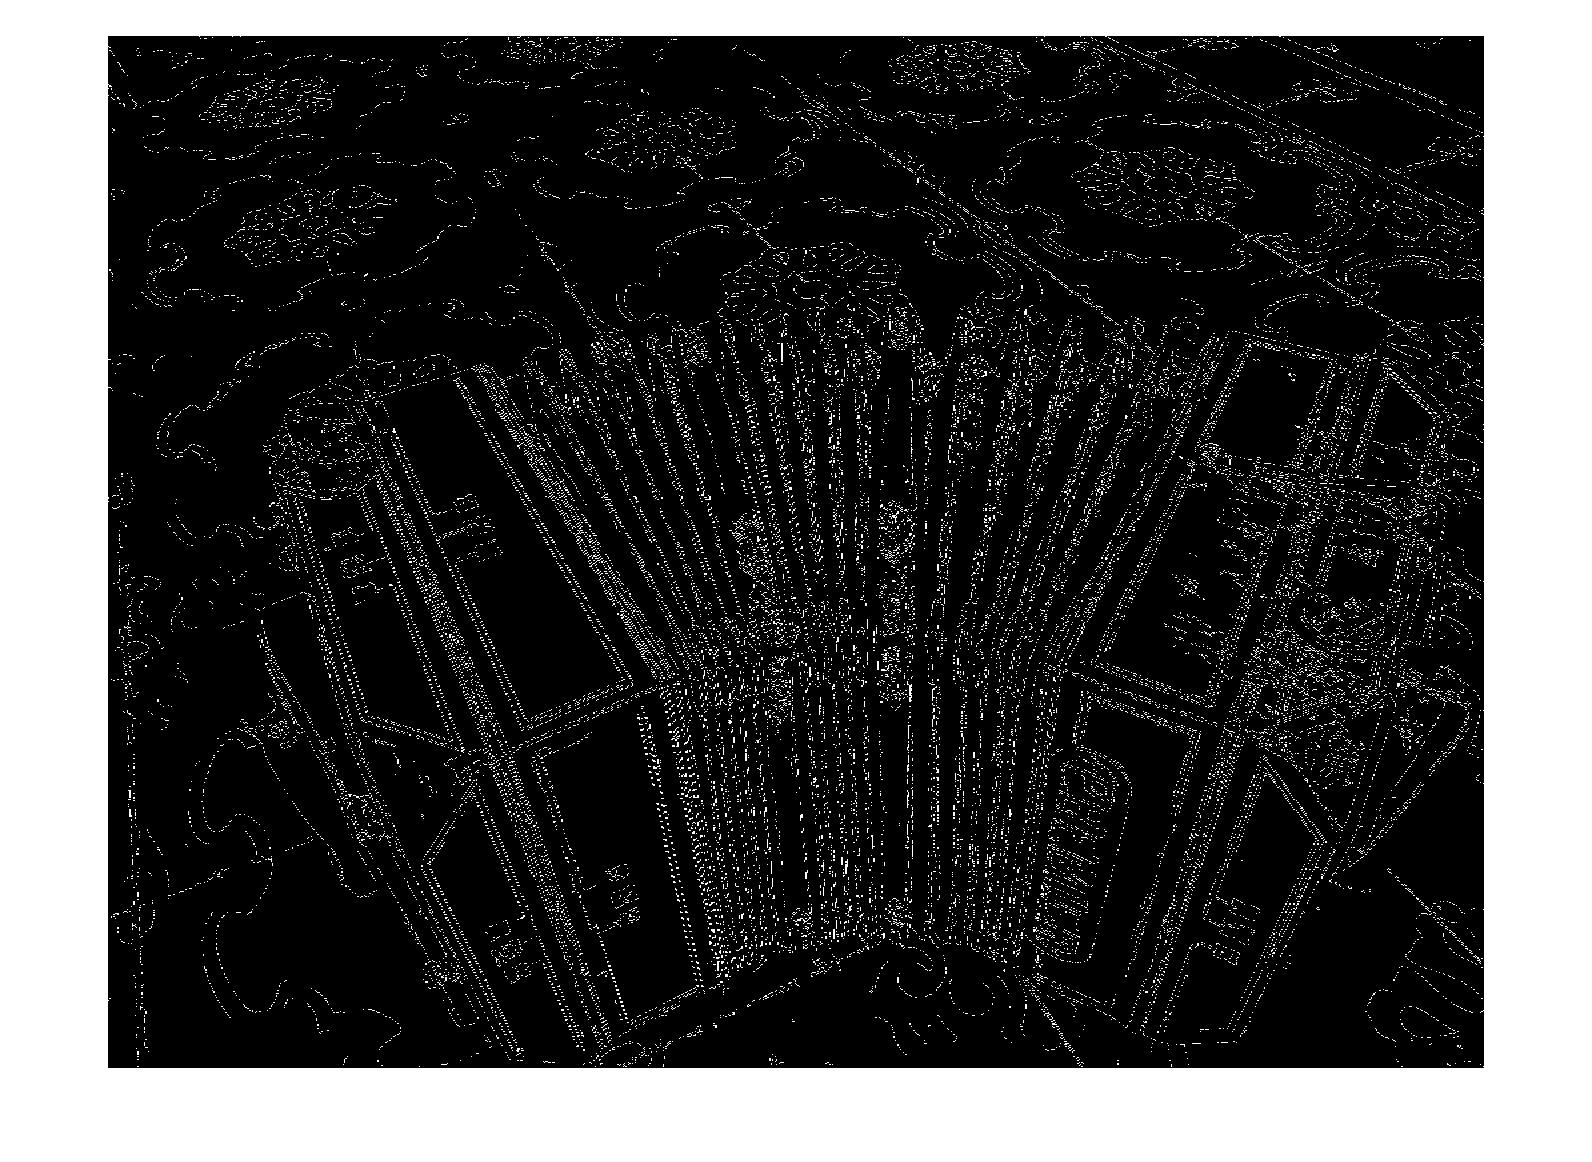
\includegraphics[width=0.8\linewidth]{edges.jpg}

\caption{Edge detection through Canny}
\label{edge}

\end{figure}

\subsection{Hough Transform} 
The Hough transform is designed to detect lines, using the parametric representation of a line:

$$rho = x*cos(\theta) + y*sin(\theta) $$

Each individual datum (edge) votes for all the model compatible with him ( $f(m,xi) = 0 $).

Steps:

\begin{itemize}
\item Discretize model space. Set the number of votes for each model = 0
\item For each datum computes the hough transform H(xi)
\item Let xi votes for each cell of the hough space crossed by H.
\item Selects the local maxima in the hough space
\item Apply a threshold to the number of votes.
\end{itemize}

The result of the application of the Hough Transform for line detection is shown in figure \ref{hough}.

\begin{figure}
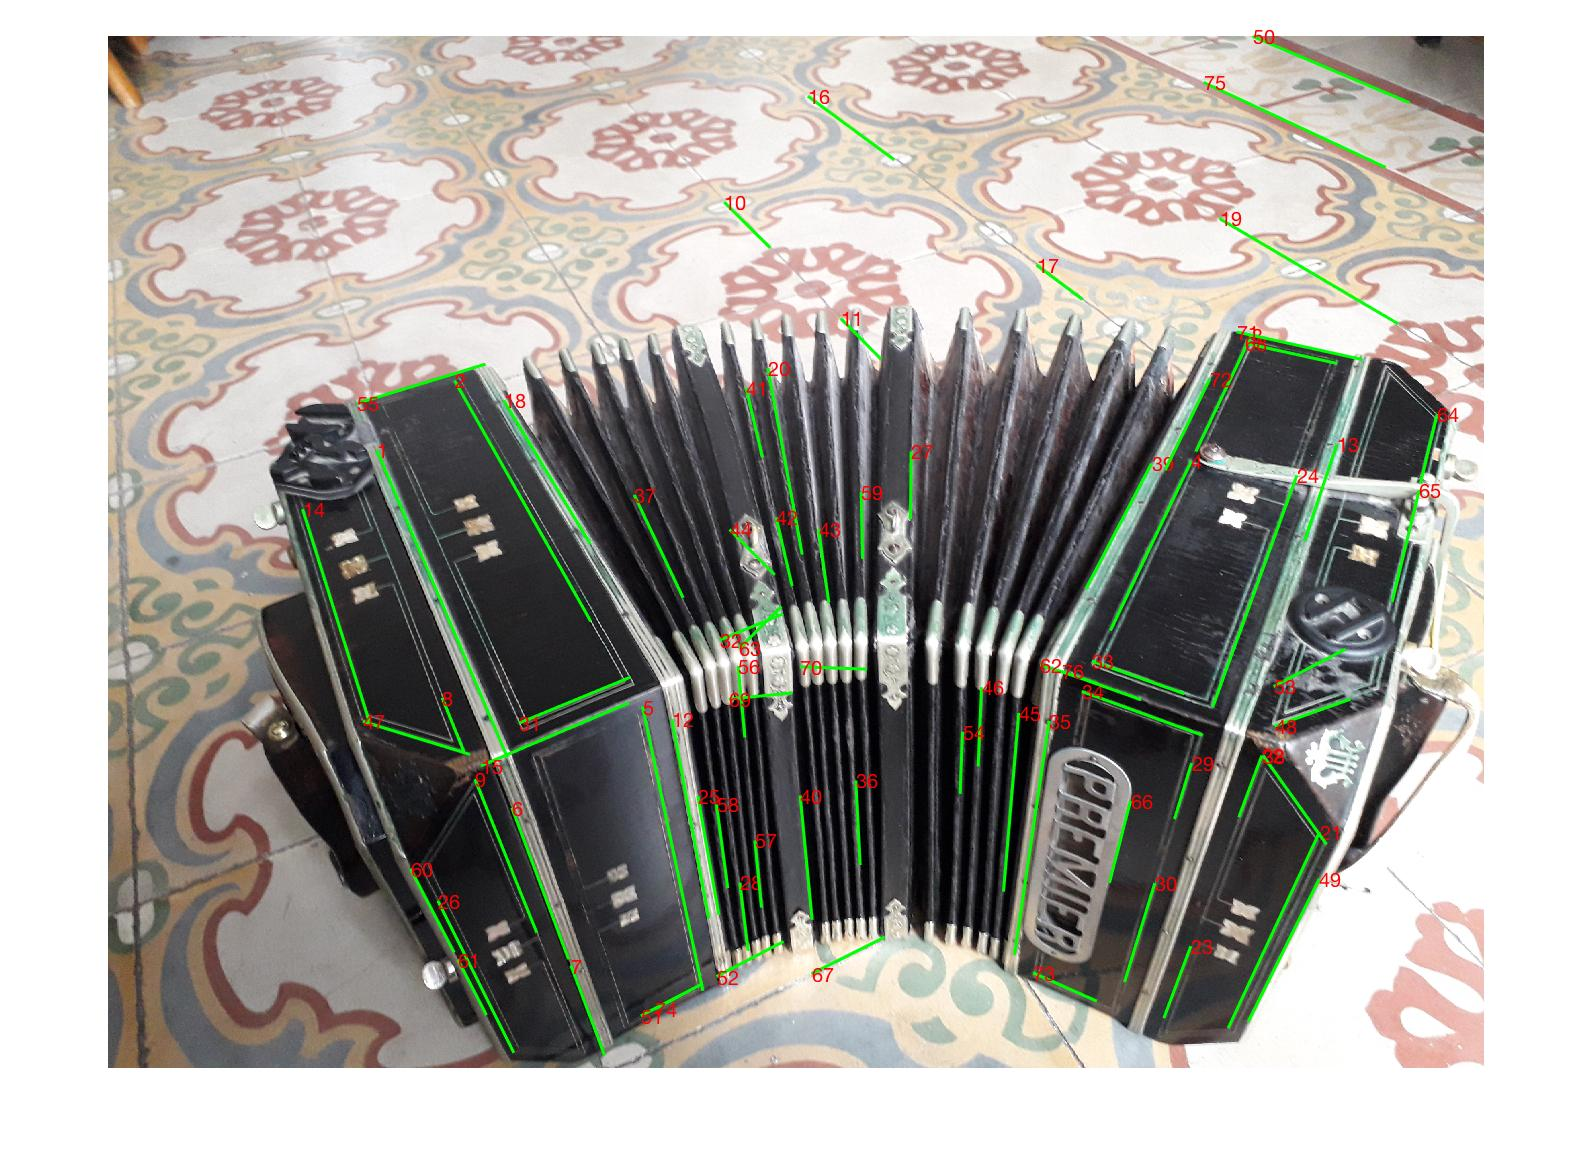
\includegraphics[width=0.8\linewidth]{lines.jpg}

\caption{Line detection through Hough}
\label{hough}
\end{figure}

\section{Shape Reconstruction}
\textbf{Using constraints on the horizontal lines, and their images, reconstruct the shape of the horizontal faces, and determine their relative position and orientation.} \hfill \break
I used a stratified approach to the shape reconstruction problem. The idea is to pass through two transformations, then the reconstructive transformation is the composition of the two transformations. 

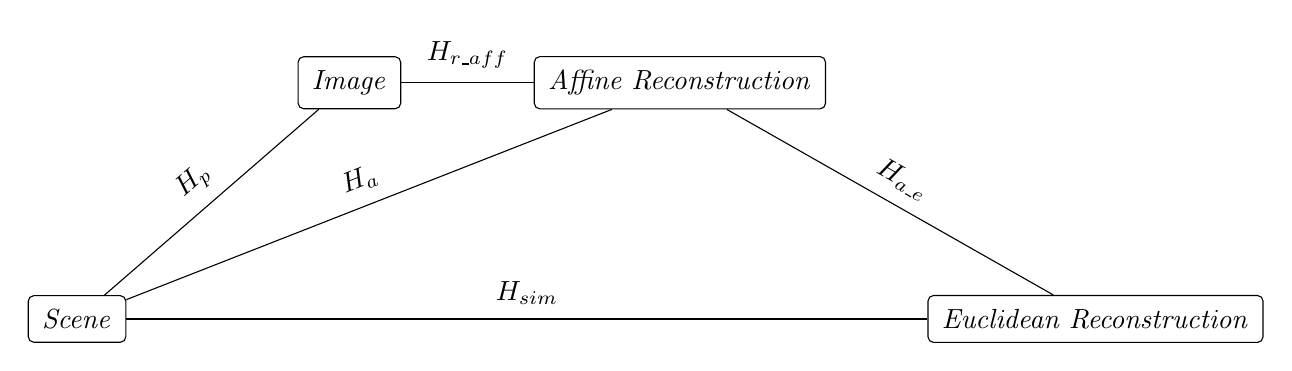
\begin{tikzpicture}[rounded corners=2pt,inner sep=5pt,node distance=0.8cm]
\node [draw](scene) at (0,0) {\textit{Scene}};
\node [draw,right=of scene] (image) at (2,3) {\textit{Image}};
\node [draw,right=of image] (affine) at (5,3){\textit{Affine Reconstruction}};
\node [draw,right=of affine] (euclidean) at (10,0) {\textit{Euclidean Reconstruction}};
\path[every node/.style={sloped,anchor=south,auto=false}]
 (scene) edge node {$H_p$} (image)
 (image) edge node {$H_{r\_aff}$}  (affine)
 (scene) edge node {$H_{a}$} (affine)
 (affine) edge node {$H_{a\_e}$}  (euclidean)
 (scene) edge node {$H_{sim}$}  (euclidean);
\end{tikzpicture}

The first step is to compute $H_{r\_aff}$ that maps the image to an affine reconstruction with respect to the real scene. Then, from the affine reconstruction compute the mapping $H_{a\_e}$ that maps the affinity to a euclidean reconstruction with respect to the real scene.

\subsection{Affine Rectification}
An affine transformation is a non-singular linear transformation followed by a translation.
Its matrix representation is the following:
\begin{equation}
\begin{bmatrix}
x' \\ y' \\ z' 
\end{bmatrix}
= 
\begin{bmatrix}
a_{11} & a_{12} & t_x \\ a_{21} & a_{22} & t_y  \\ 0 & 0 & 1
\end{bmatrix}
\begin{bmatrix}
x \\ y \\ 1
\end{bmatrix}
\end{equation}
Because an affine transformation includes non-isotropic scaling, the similarity invariants of length ratios and angles between lines are not preserved under an affinity.
Invariants of an affinity are:
\begin{itemize}
\item Parallel lines. An affine transformation maps points at infinity to points  at infinity. Consequently, the parallel lines are mapped to lines which still intersect at infinity, and so are parallel after the transformation.
\item Ratio of lengths of parallel segments
\item Ratio of ares
\end{itemize}

In order to perform affine rectification we require that the line at infinite in the image is mapped back to itself ($l_{\infty} = (0,0,1)^{T}$).
So we first perform the identification of the imaged line at infinite through LSA using n couples of imaged parallel lines. 
Once found the image of the line at infinite the reconstruction matrix that rectifies the image it's simply:

\begin{equation}
H_{r\_aff} =\begin{bmatrix} 
1& 0 & 0 \\
0 &  1 & 0 \\
l_1 &  l_2 & l_3 \\
\end{bmatrix}
\end{equation}

So the last row is the imaged line at infinite [pag 49 Multiple View Geometry in computer vision].

The result of the affine rectification on the input image is in figure  {\ref{affine}}.

It's possible to see that parallel lines are now parallel, even if angles do not show their real value.

\begin{figure}
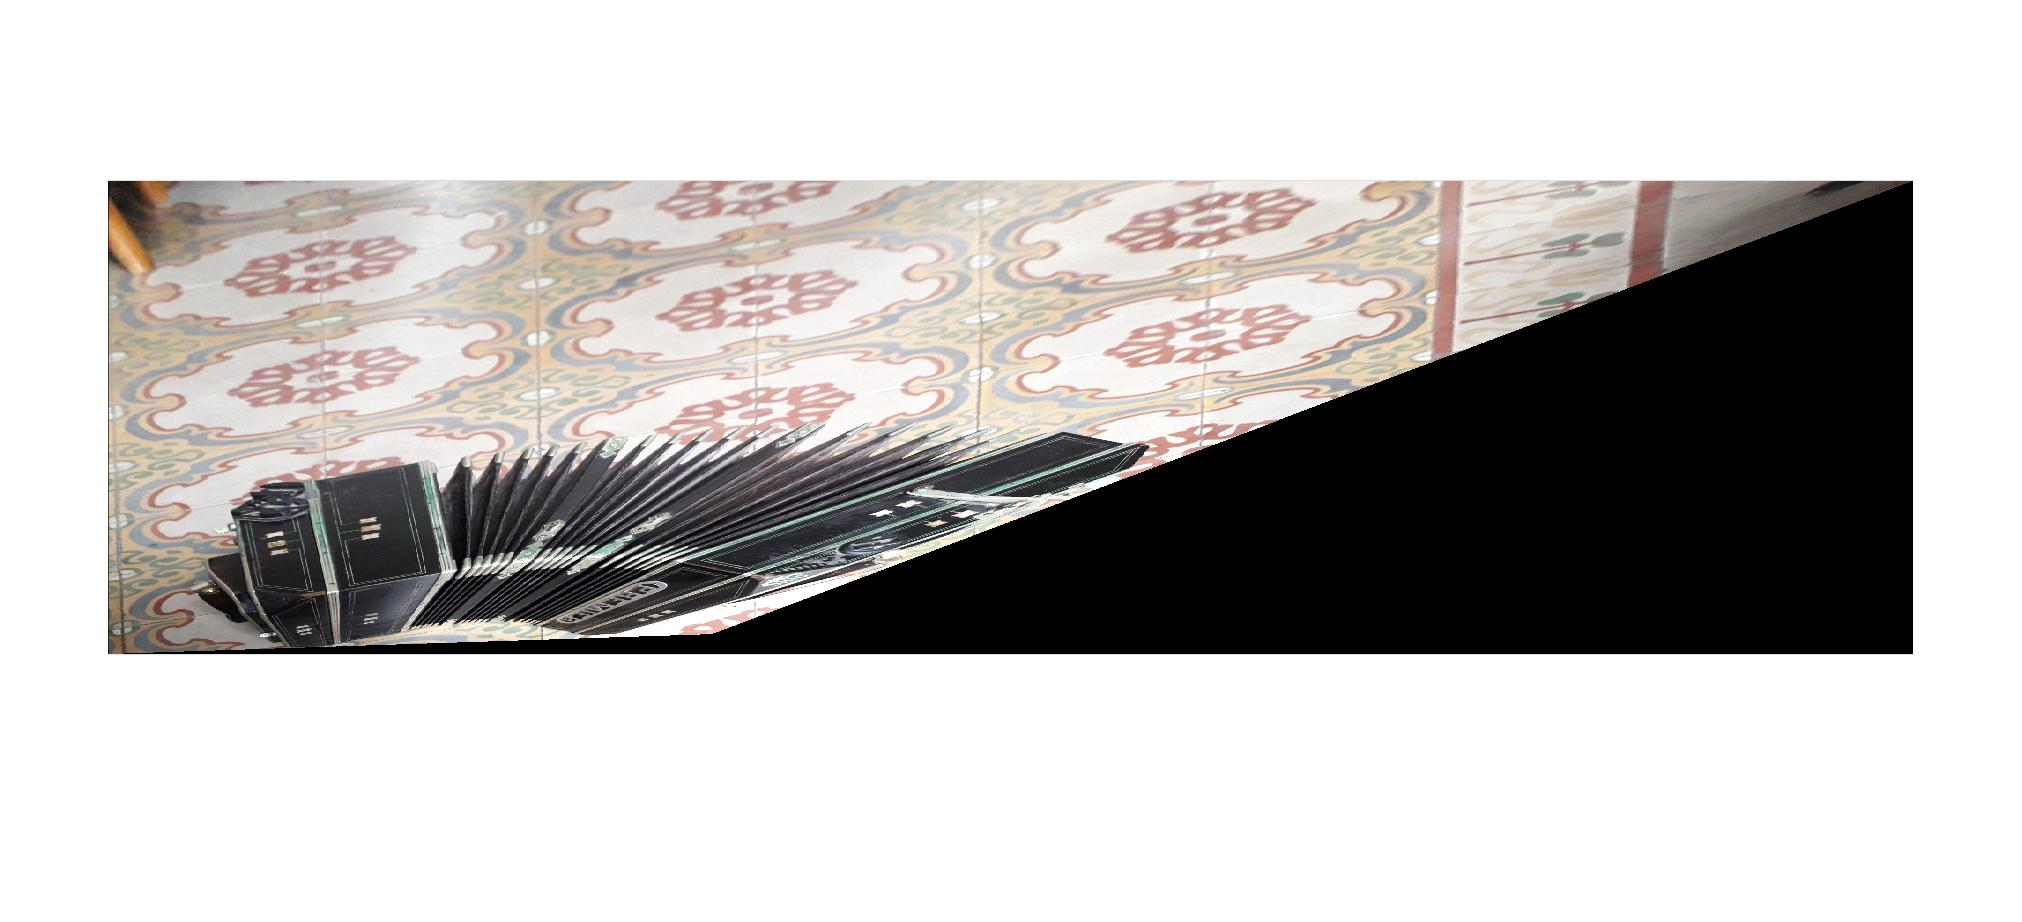
\includegraphics[width=0.8\linewidth]{rectified_img.jpg}
\caption{Affine rectification}
\label{affine}
\end{figure}

\subsection{Euclidean Rectification}
A similarity transformation (or more simply a similarity) is an isometry composed with an isotropic scaling. In the case of a Euclidean transformation composed with a scaling (i.e. no reflection) the similarity has matrix representation:
\begin{equation}
\begin{bmatrix}
x' \\ y' \\ z'
\end{bmatrix}
=
\begin{bmatrix}
s \cos\theta & - s \sin\theta & t_x \\ s \sin\theta & s \cos\theta & t_y \\ 0 & 0 & 1
\end{bmatrix}
\begin{bmatrix}
x \\ y \\ 1
\end{bmatrix}
\end{equation}

where the scalar s represents the isotropic scaling.
A similarity transformation preserves the shape of objects.
Invariants:
\begin{itemize}
\item Angles between lines (and parallel lines)
\item Ratio of lengths
\item Ratio of areas
\end{itemize}

Once the image has been affinely rectified we have obtained an image such that the transformation from the original scene is an affine transformation.
The image of the dual conic corresponding to circular points can be obtained as:
\begin{subequations} \label{shapereceq}
\begin{align}
C^*_{\infty}{'} & = H_a C^*_{\infty} H_a^t  \\
C^*_{\infty}{'} & = \begin{bmatrix} 
a_{11}^{2} & a_{12}*a_{21} & 0 \\
 a_{12}*a_{21} &  a_{22}^{2}  & 0 \\
0 &  0 & 0 \\
\end{bmatrix} \\
 C^*_{\infty}  & = H_a ^{-1} C^*_{\infty}{'} H_a ^{-t}
\end{align}
\end{subequations}
Notice that the upper left part of $C^*_{\infty}{'} $ is a symmetric matrix and homogeneous, so it has only 2 DOF.
We can use two pair of orthogonal lines, $l$ and $m$, to determine its parameters using equation \ref{coseq}.
\begin{subequations} \label{coseq}
\begin{align}
\cos(\theta) & = \frac{l_1 m_1 + l_2  m_2}{\sqrt{(l_1^2 + l_2^2)(m_1^2 + l_2 ^2)}}  \\
\cos(\theta) & = \frac{l C^*_{\infty} m} {\sqrt{(l^t C^*_{\infty} l) (m^t C^*_{\infty} m)}} \\
\cos(\theta) & = \frac{l' C^{*}_{\infty}{'} m'} {\sqrt{(l^{'t} C^{*}_{\infty}{'} l') (m^{'t} C^{*}_{\infty}{'} m')}}
\end{align}
\end{subequations}
That, in the case of orthogonal lines, becomes a linear constraint on $C^{*}_{\infty}{'}$.

The matrix $H_a$ in equation \ref{shapereceq} is the transformation matrix from the real scene to the image, so the matrix $H_a^{-1}$ is the matrix that maps the image to a similarity with respect to the real scene since the matrix $C^*_{\infty} $ is mapped back to its value.

Once found $C^*_{\infty}{'}$ we can use standard cholesky (or SVD) to determine $H_a$:
$$
svd(C^*_{\infty}{'}) = USV^{t} = H_a C^*_{\infty} H_a^t 
$$
Where $H_a = U$.
Since SVD does not return the matrix S ($C_{\infty}^*$) as 
$$C_{\infty}^* = \begin{bmatrix} 1 & 0 & 0 \\ 0 & 1 & 0 \\ 0  & 0 & 0\end{bmatrix} $$
that is required by the algorithm, it's possible to factorize the matrix S returned by SVD through the following decomposition:

\begin{subequations}
\begin{align*}
S & = S_{fact} C_{\infty}^* S_{fact} \\
S & = \begin{bmatrix} \sqrt{S_{11}} & 0& 0 \\ 0 & \sqrt{S_{22}}  & 0   \\ 0 & 0 & 1 \end{bmatrix} \begin{bmatrix} 1 && \\&1&\\&&0\end{bmatrix} \begin{bmatrix} \sqrt{S_{11}} & 0& 0 \\ 0 & \sqrt{S_{22}} & 0   \\ 0 & 0 & 1 \end{bmatrix} 
\end{align*}
\end{subequations}

Doing in this way the factorization of $C^*_{\infty}{'}$ becomes:

$$
C^*_{\infty}{'} = USV^{t} = U S_{fact} C_{\infty}^* S_{fact} V^{t} = H_a C^*_{\infty} H_a^t 
$$

In this way the matrix $H_a$ becomes:
$$
H_a = U S_{fact}
$$
Renaming the matrix $H_a^{-1}$ as $H$  the overall transformation ($H_r$, reconstructive matrix) that maps the image to a similarity is the composition of the two transformation:
$$
H_r = H H_{r\_aff} 
$$

The final result of the shape reconstruction phase for the two upper faces is showed in figure \ref{shaperec}.

\begin{figure}
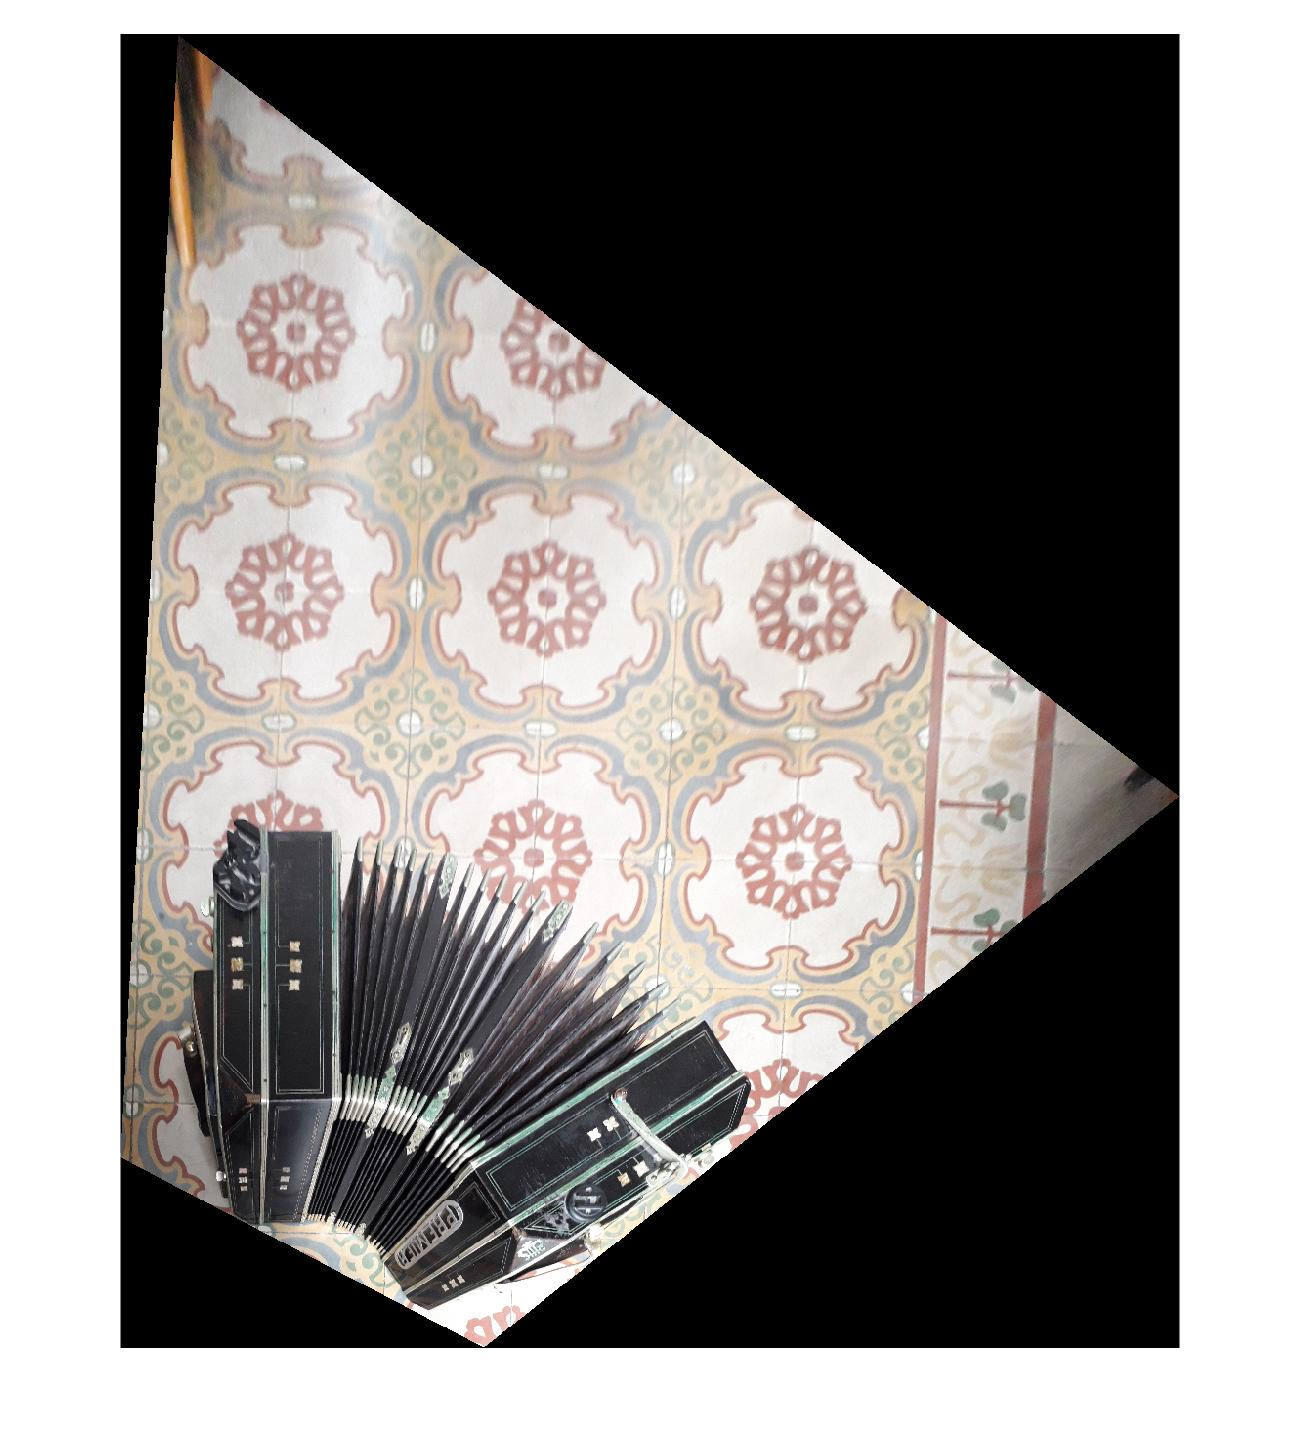
\includegraphics[width=0.8\linewidth]{shape_rec_rotated.jpg}
\caption{Shape reconstruction}
\label{shaperec}
\end{figure}

\section {Measure of Metric Properties} \label{metricprop}
Once we have reconstructed the shape of the object, metric properties can be determined, like angles, since they are invariants of a similarity transformation.

The relative orientation between the horizontal upper faces can be determined using the cosine between the two lines representing corresponding lines in each face.

Given two corresponding lines in each faces the cosine between them can be determined using equations \ref{coseq}.

The relative position can be determined simply by computing the difference between the origin of the two reference frames and multiplying by the scaling factor.
The scaling factor can be determined by doing the ratio between the length of the longside of the horizontal face and the length in the image of the corresponding side.
The relative position estimated as before gives us the relative position in the reference frame of the image. If we want the position of the right face with respect to the left face in the reference frame of the left face we need to multiply the rotation matrix of the reference frame of the left face and the vector of the relative positions:
$$
relative\_pose\_from\_left\_to\_right = R_{from\_img\_to\_left} * relative\_coordinates
$$
\section{Camera Calibration} 
\textbf{Using also the images of vertical lines, calibrate the camera (i.e., determine the calibration matrix K) assuming it is zero-skew (but not assuming it is natural).} \hfill \break

Camera calibration is determining the matrix K of the intrinsic parameters of the camera:

\begin{equation} \label{keq}
K =
\begin{bmatrix}
f_x  && 0 && u_0 \\ 0 && f_y && v_0 \\ 0 && 0 && 1
\end{bmatrix}
\end{equation}

P is the projection matrix that maps 3d points (X) of the world to points in the image (x) through the relation:
\begin{equation} \label{peq1}
x = P X
\end{equation}
Where P is the matrix:
\begin{equation} \label{peq}
P=[KR | -KRo]
\end{equation}
In equation \ref{peq}, R is the rotation between the camera and the world (represents the rotation of the camera with respect to the world reference frame) and o is the location of the camera in the world reference frame.

K is related to $\omega$ through the following equation:

$$
\omega = (KK^t)^{-1}
$$

In order to determine K we need to specify some constraints on $\omega$ (the image of the absolute conic).

For a zero skew camera the image of the absolute conic is given by

\begin{equation} \label{omegaeq}
\omega = 
\begin{bmatrix}
\alpha^2 && 0 && -u_0 \alpha^2 \\ 0 && 1 && -v_0 \\  -u_0 \alpha^2 && -v_0 && f_y^2 +\alpha^2 u_0^2 + v_0^2
\end{bmatrix}
\end{equation}
That is a symmetric matrix with 4 DOF, so we need 4 constraints on $\omega$.
Here we can use the homography method (p 211 Multiple View Geometry in Computer Vision) adapted with the reconstructive transformation (that we have found in the previous point) on the horizontal faces.

\begin{itemize}
\item For each horizontal face we can compute the transformation that maps its corner points to their imaged points ($H_r^{-1}$ since $H_r$ maps the image point to their real shape).
\item We can compute the imaged circular points for the plane of that face as $H_r(1,\pm i, 0)'$. Writing $H_r$ = [h1, h2, h3], the imaged circular points are $h1 \pm ih2 $.
\item This gives us two constraints on the image of the absolute conic since the circular points lie on $\omega$:

   \begin{subequations}
   \begin{align*}
   & h_1^T\omega h_2= 0 \\ 
   & h_1^T\omega h_1= h_2^T\omega h_2 
   \end{align*}
   \end{subequations}
   Which are linear equations in $\omega$.

\end{itemize}
Other constraints that can be used are the constraints deriving from the fact that the line at infinity on the horizontal plane is orthogonal with respect to the vanishing point of the vertical direction on the vertical faces:
$$
l_{inf}^T\omega v_p = 0
$$

In order to determine the vanishing point of the vertical direction we can use a least square approximation using all vertical lines on the vertical face.
Once having determined $\omega$ it's possible to obtain the calibration matrix K using the parametrization in equation \ref{omegaeq}. 

\section{Localization}
\textbf{ Localize the camera with respect to (both) horizontal faces. From the image of the (short) horizontal segments common to a horizontal face and its neighboring vertical face, reconstruct the shape of the vertical faces.} \hfill \break
In this point we have to find the relative position of the camera with respect to the reference frame placed on the horizontal faces.

This is possible knowing the shape of the horizontal faces, knowing the size, knowing the image and knowing K.

If we identify the plane of the left horizontal face with $\pi$ we can write the position of a point in the world reference frame as $ X_w =[R_{\pi} | o_{\pi}]X_{pi} $ where $X_{pi} $ is the position of the point in the plane reference frame. Using equations \ref{peq1} and \ref{peq} we obtain:

$$
u = [KR | -KRo] [R_{\pi} | o_{\pi}]X_{pi}
$$

By putting the world reference frame on the camera ($R=I$ and $o=[0 \ 0\ 0\ 1]'$):

\begin{subequations}
\begin{align*}
u  & = [K|0][i_\pi | j_\pi | o_\pi] \begin{bmatrix}
x \\ y \\ w
\end{bmatrix} \\
u & = K [i_\pi | j_\pi | o_\pi] x
\end{align*}
\end{subequations}
Where x are the coordinates of the point on the plane. 
By inspection we can identify $K [i_\pi | j_\pi | o_\pi] = H_omog$ as the matrix that maps the real points to the image. H is known since the shape of horizontal face is known and also its size.

So we obtain:

$$[i_\pi | j_\pi | o_\pi]= K^{-1}H_omog $$

Where $H_omog$ is the transformation mapping world points to image point. 

$H_{omog}$ it's easy to find since knowing the shape it's the transformation that maps the shape of the horizontal face to the image. 

A few more steps are needed once found the matrix $H_{omog} = [h_1\; |\; h_2\; |\; h_3]$. 

The matrix $R=[i_\pi\; | \; j_\pi \; | \; k_\pi]$ (rotation of the plane with respect to the camera) can be found using these equations:

\begin{subequations}
\begin{align*}
\lambda &= \frac{1}{|K^{-1}h_1|} \\
i_\pi &= K^{-1}h_1\lambda \\
j_\pi &= K^{-1}h_2\lambda \\
k_\pi &= i_\pi \times j_\pi  \\
o_\pi &= K^{-1} h_3 \lambda
\end{align*}
\end{subequations}

Due to noise in the data R may be not a true rotation matrix, it's possible to approximate it through SVD, obtaining an orthogonal matrix:

\begin{subequations}
\begin{align*}
[U,\; \_\;,\;V] &= svd(R) \\
\hat{R} &= UV
\end{align*}
\end{subequations}

The result of the camera localization phase is shown in figure \ref{left_loc}.

\begin{figure}
 \centering
    \subfloat{{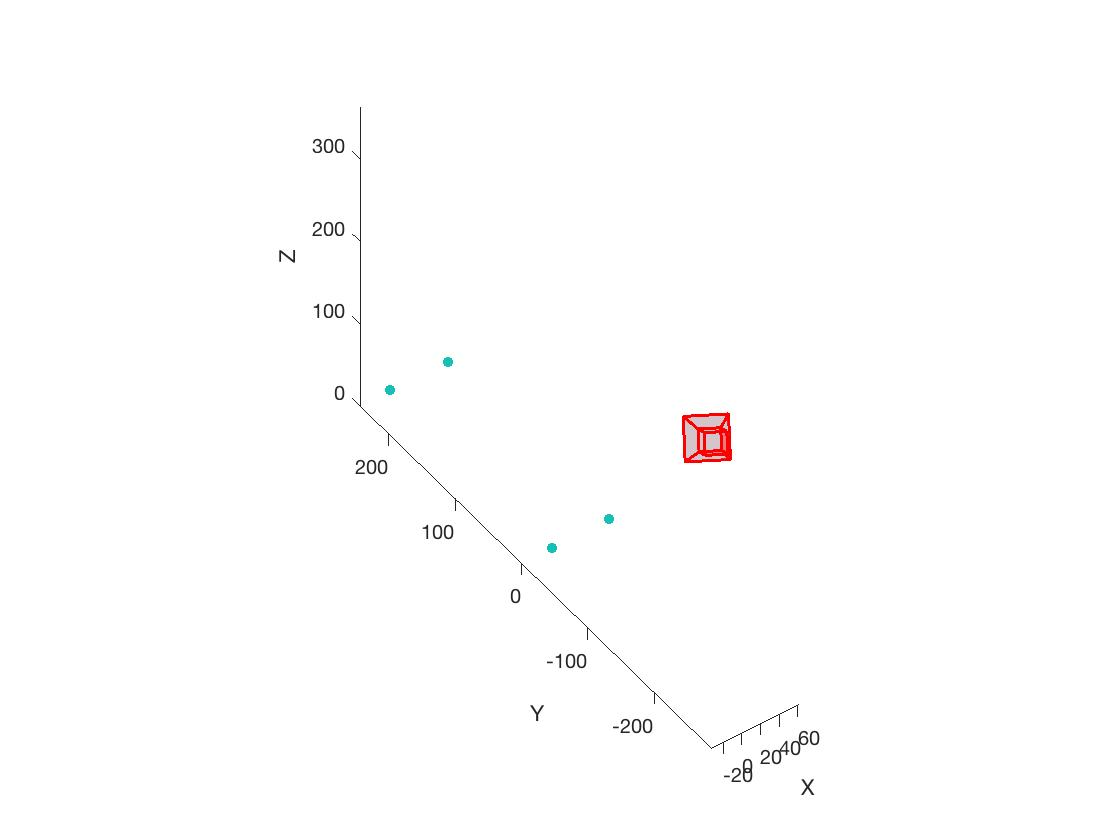
\includegraphics[width=5cm]{left_loc.jpg} }}%
    \qquad
    \subfloat{{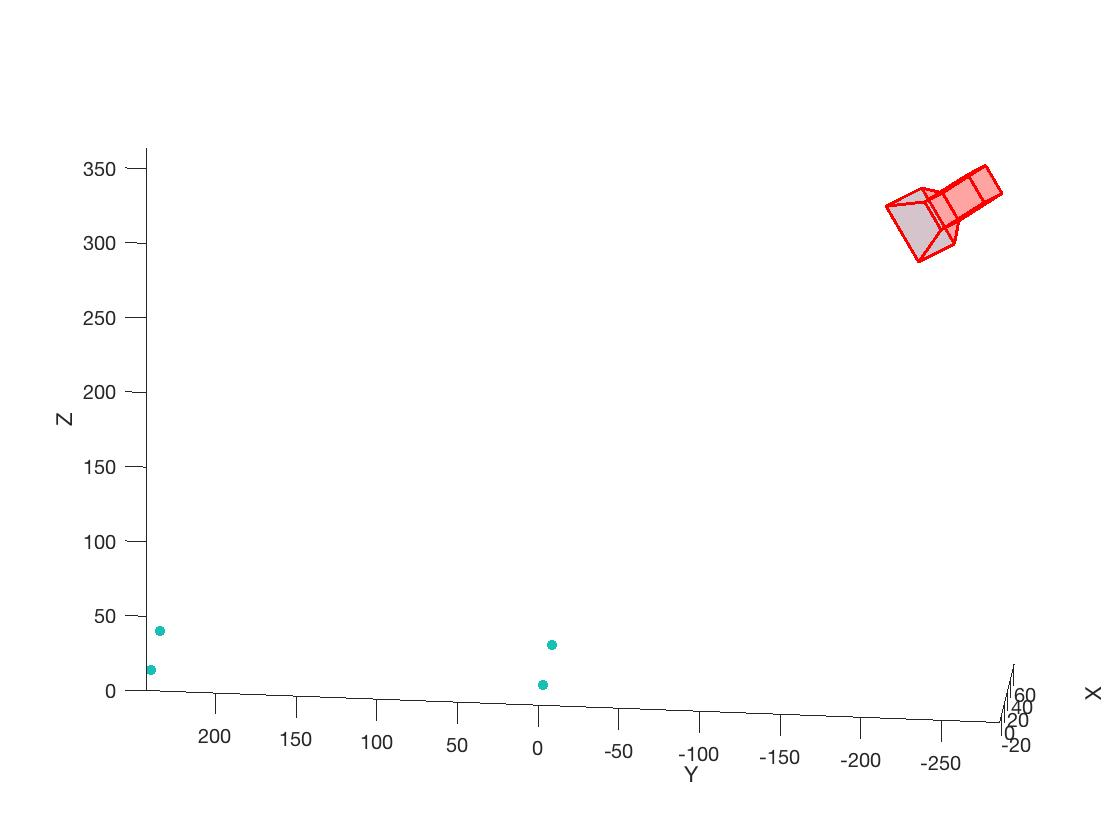
\includegraphics[width=5cm]{left_loc2.jpg} }}%
    \caption{Camera Localization from left face}%
    \label{left_loc}%
\end{figure}

The rotation of the right plane can be found simply by applying the rotation found in section \ref{metricprop}.

$$
R_{right} = \hat{R}*R\_from\_left\_to\_right
$$

\begin{figure}
 \centering
    \subfloat{{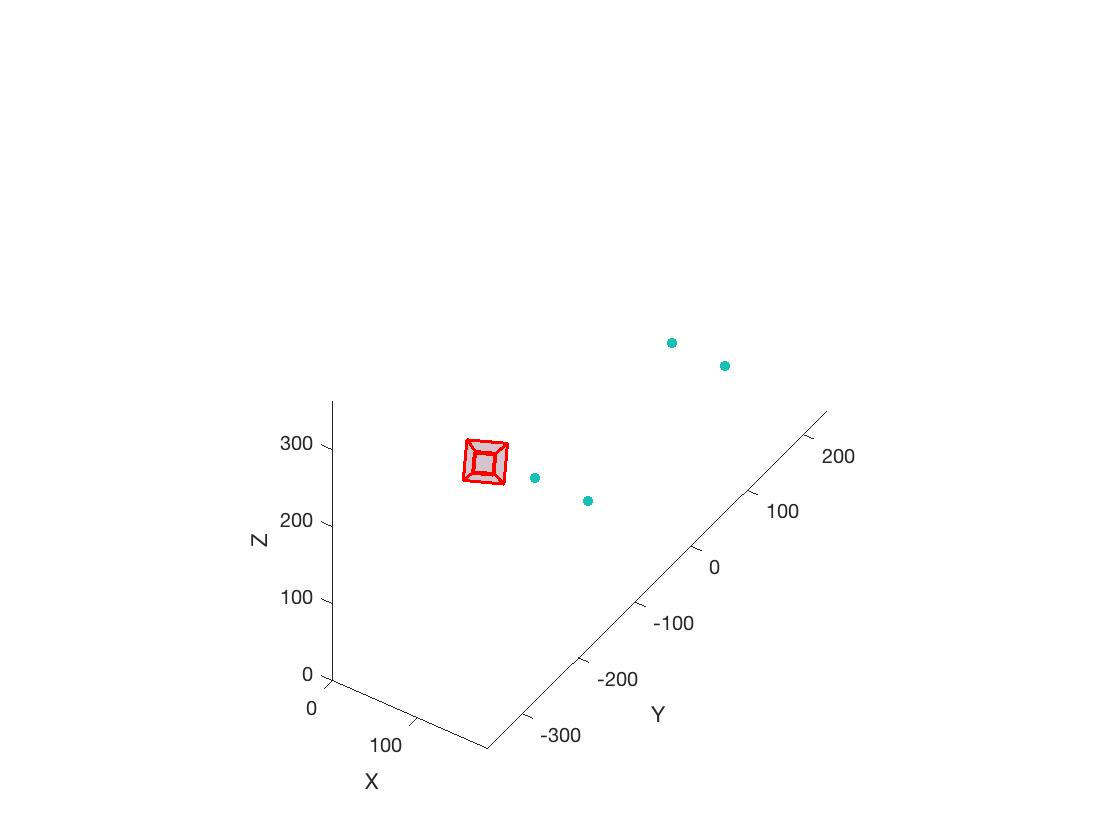
\includegraphics[width=5cm]{right_loc.jpg} }}%
    \qquad
    \subfloat{{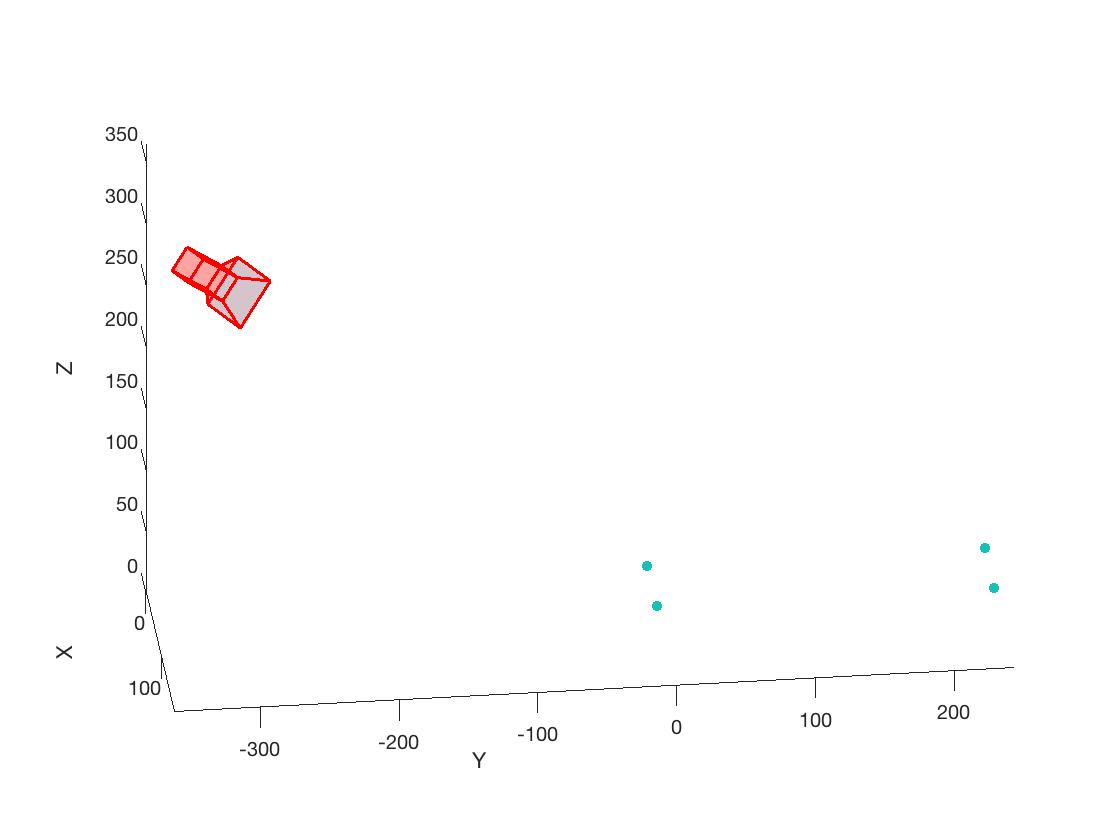
\includegraphics[width=5cm]{right_loc2.jpg} }}%
    \caption{Camera Localization from right face}%
    \label{right_loc}%
\end{figure}

\begin{figure}
 \centering
    \subfloat{{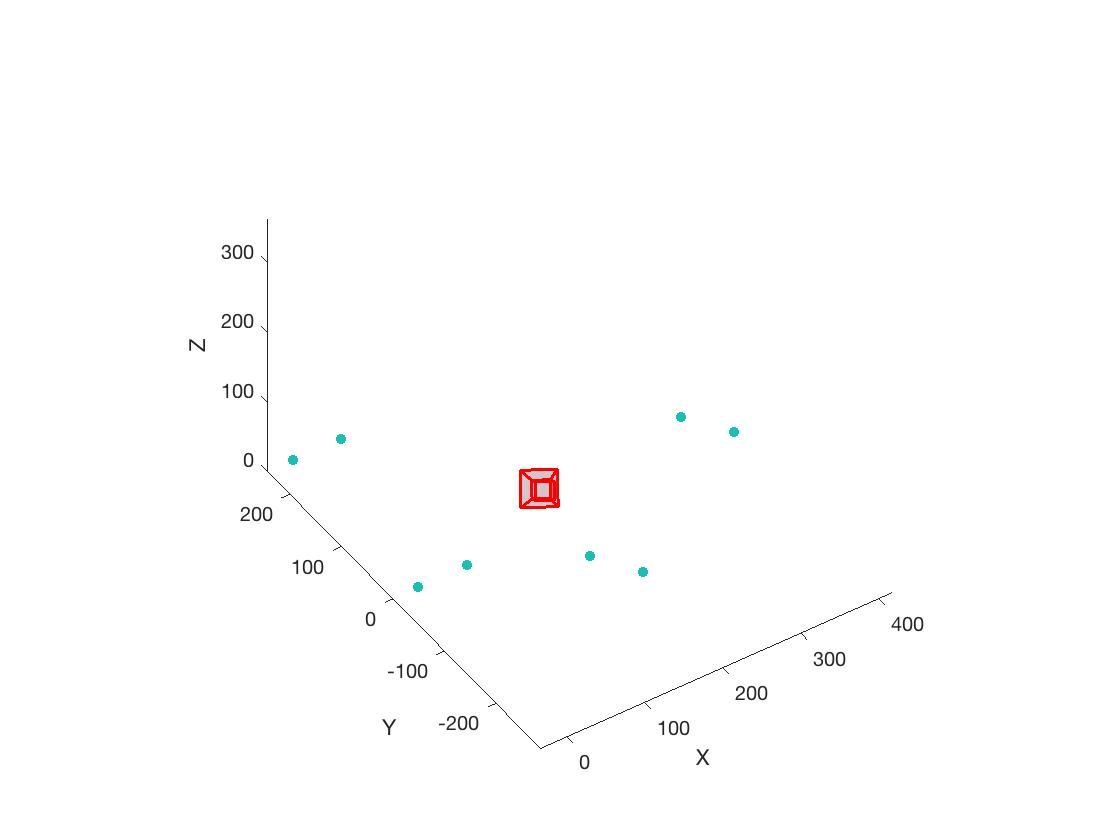
\includegraphics[width=5cm]{general_loc.jpg} }}%
    \qquad
    \subfloat{{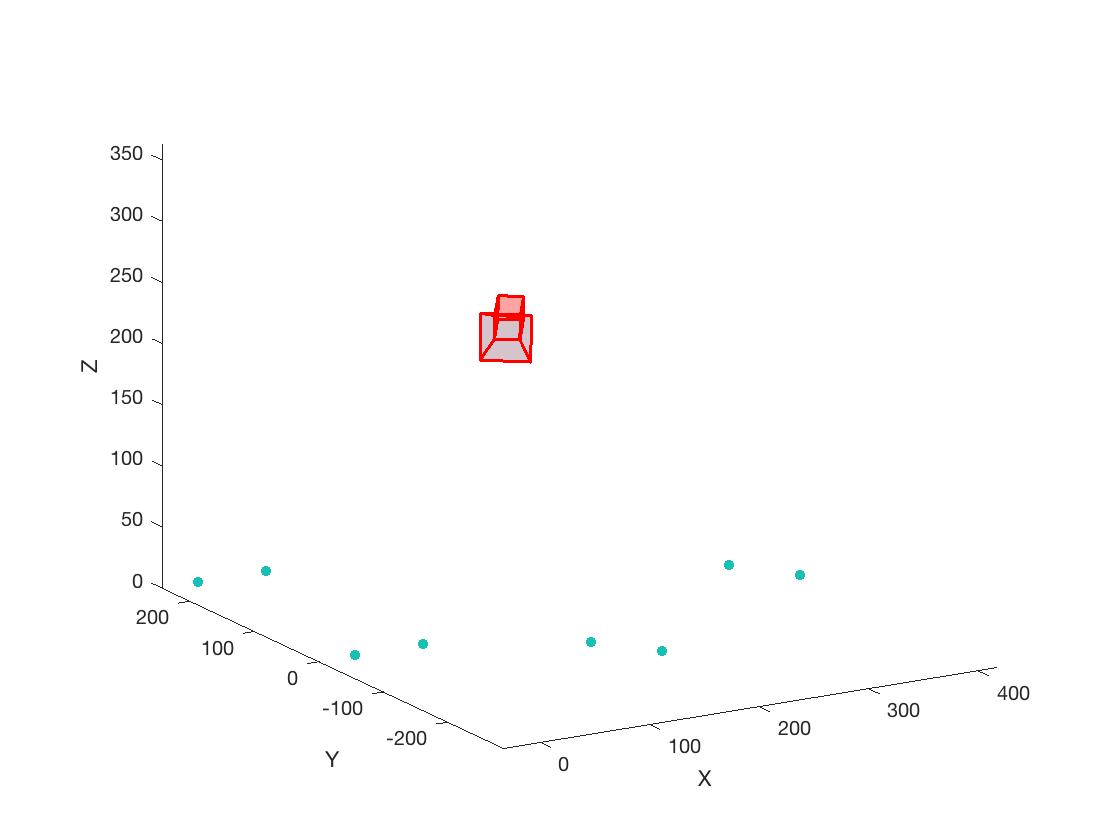
\includegraphics[width=5cm]{general_loc2.jpg} }}%
    \caption{Camera Localization from both face}%
    \label{general_loc}%
\end{figure}

\section{Shape Reconstruction Vertical Faces }
For the shape reconstruction of vertical faces we can use the result of the localization, namely the matrix R, the rotation of the plane with respect to the camera.
If we put the world reference frame on the horizontal face we obtain the following matrix P:
$$ P = [K \hat{R} / \lambda\  | \ o_\pi / \lambda] $$
The elementwise division by lambda is needed to reconstruct the original ratios.
The reference frame of the vertical face it's the same of the horizontal face, a point on the vertical face has always $y=0$ and the z has the inverse sign.
The matrix P maps the point on the vertical face to image points so we can directly use the matrix $ H_{vert\_sr} = [p_1 \; |\; p_3 \;|\; p_4]^{-1}$ to reconstruct the shape of the vertical left face.
The reconstruction of the vertical right face can be performed in the same way using the matrix $R_{right}$.
The reconstructed  vertical faces are shown in figure \ref{verticalshaperec}.

\begin{figure}
 \centering
    \subfloat{{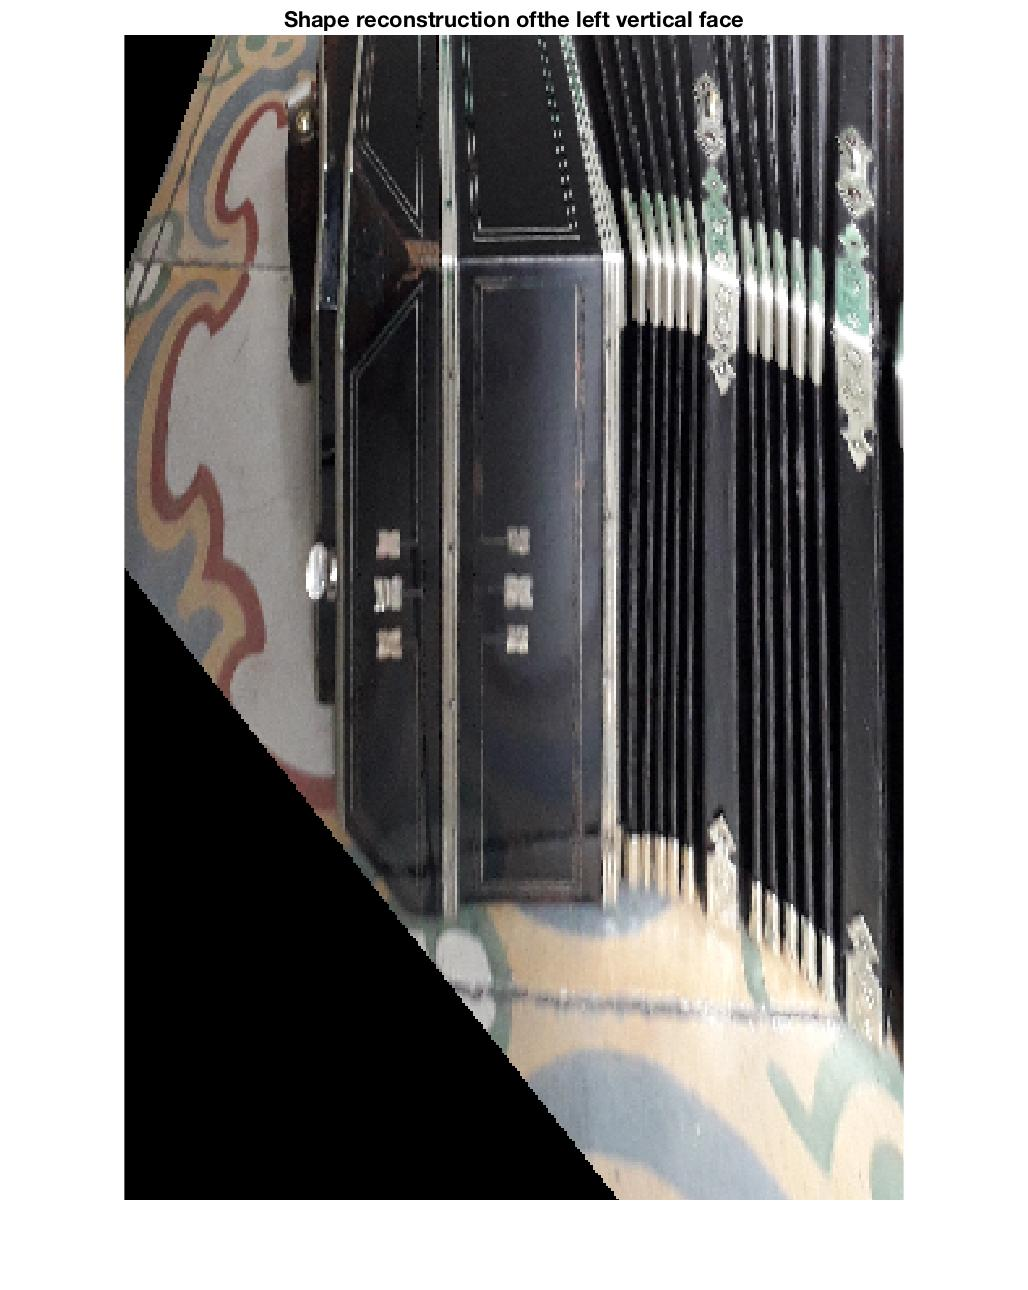
\includegraphics[width=5cm]{vertical_face_left.jpg} }}%
    \qquad
    \subfloat{{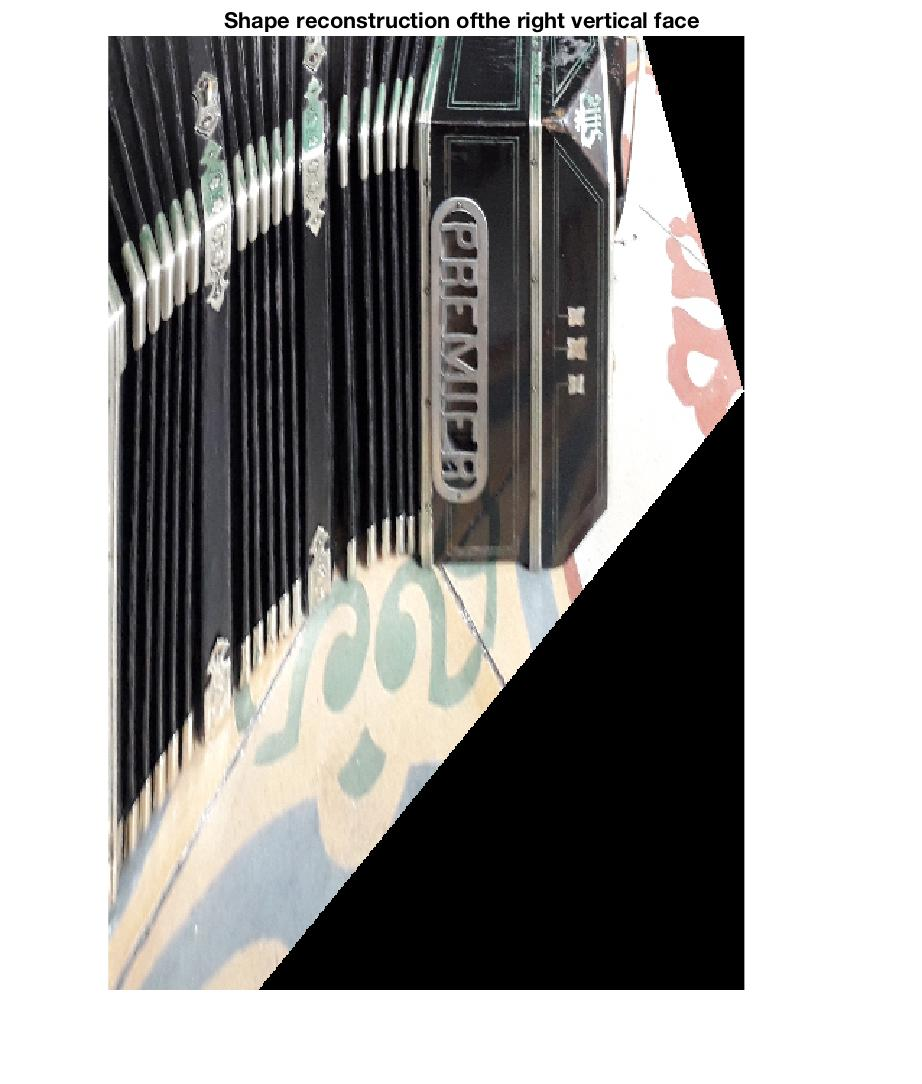
\includegraphics[width=5cm]{vertical_face_right.jpg} }}%
    \caption{Shape Reconstruction of the vertical faces}%
    \label{verticalshaperec}%
\end{figure}

\section{Implementation Details}
In this section implementation details are explained.
\subsection{Vanishing Points}
Vanishing points are extracted using a Least Square Approximation:
A vanishing point is a point common to all line having the same direction. 
Considering the line $l$ as data and the vanishing point $v$ as model:
\begin{subequations}
\begin{align*}
f(l,v)&=0 \\
l'v &= 0
\end{align*}
\end{subequations}

Considering the vanishing point with 2DOF ($v_3=1$), the equation becomes:

$$
l_1 v_1 + l_2 v_2 = -l_3
$$

It's possible to rephrase this in a model fitting framework using these matrices:
$$
X = \begin{bmatrix}
l_{11} && l_{21} \\
\vdots  && \vdots\\
l_{1n} && l_{2n}
\end{bmatrix}
$$ 

$$
W = 
\begin{bmatrix}
v_1 \\
v_2
\end{bmatrix}
$$

$$
Y =
\begin{bmatrix}
-l_{31} \\
\vdots \\
-l_{3n}
\end{bmatrix}
$$
The solution ($W$) minimizing the error ($|Y-XW|^2$) is then found simply using:

$$
W = (X'X)^{-1}(X'Y)
$$

\subsection{Line at Infinity}
The line at infinity on the horizontal face is extracted using these steps:
\begin{itemize}
\item Vanishing point extraction using lines on the horizontal faces and on the ground. 
\item Line fitting using Least Square Approximation.
\end{itemize}


\end{document}  